\documentclass[a4paper,10pt]{article}
%\documentclass[preview=false]{standalone}
% %%%% Define new conditional \ifplastex
% %%%% This ensure that the file complied normally without plasTeX.
\usepackage{plastex}

\ifplastex\else
\usepackage{standalone} %%%% Only load standalone when not in plasTeX
\standalonetrue
\fi

% % Package for typesetting URLs
\usepackage{url}

\usepackage{import}

\usepackage{iumlb}

\usepackage{multirow}

% Package for including figures
\usepackage{graphicx}

% Package for sub-floats (e.g. figures)
\usepackage{subfig}

% % Title
\title{iUML-B Class Diagrams User Manual} 

% % Author
\author{Colin Snook\\University of Southampton}

% % Date
\date{%
	Version 0.0.1\\%
	\today%
}

\begin{document}
	\ifplastex%
	\maketitle% Make title if in plasTeX mode.
	\else%
	\ifstandalone%
	\maketitle % Make title if in standalone mode.
	\else%
	\fi%
	\fi%
	
iUML-B Class diagrams are used to visualise and model data in an entity relationship style.
Class Diagrams provide a way to model data as sets (classes) of objects.
Elements of the class diagram (class, attribute, association) \emph{elaborate} (i.e. link to) a data item (Carrier Set, Constant, Variable) in the Event-B.
The class diagram translator generates properties such as axioms or invariants in the relevant context or machine.
Linking to an existing data element, rather than create a new one, allows more flexibility.
The elaborated data item must be in-scope via sees or extends as shown in Figs.~\ref{fig:CDContainment1}, \ref{fig:CDContainment2} and 	\ref{fig:CDContainment3}.
	
	\begin{figure}[!htbp]
		\centering
		\ifplastex
		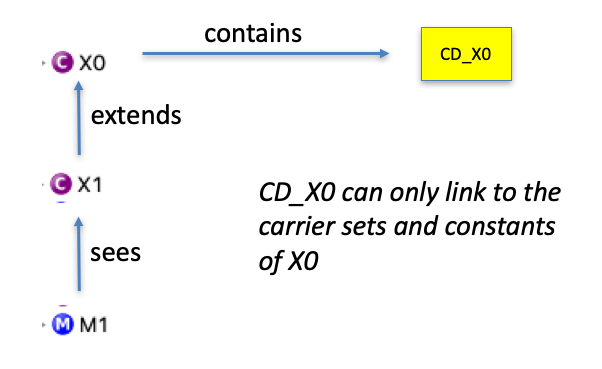
\includegraphics[width=500]{figures/containment_1.png}
		\else
		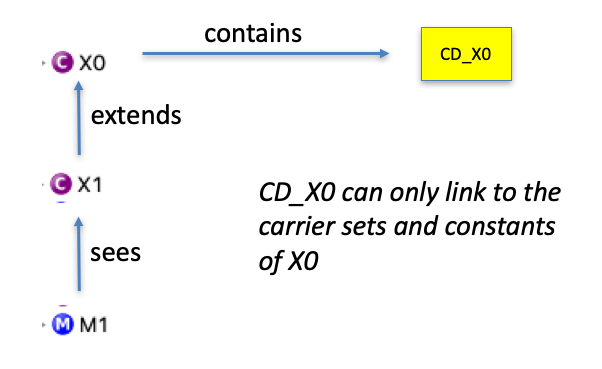
\includegraphics[width=.5\textwidth]{figures/containment_1.png}
		\fi
		\caption{Class Diagram contained in a base level Context}
		\label{fig:CDContainment1}
	\end{figure}
	
	
	\begin{figure}[!htbp]
		\centering
		\ifplastex
		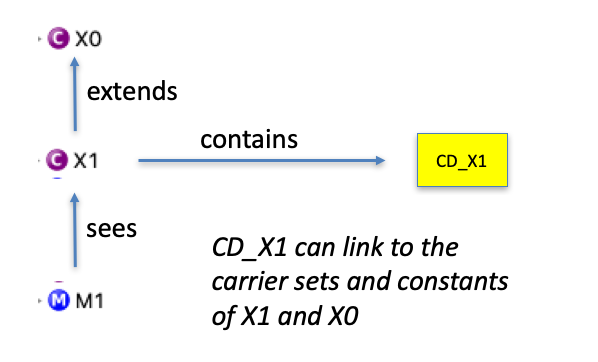
\includegraphics[width=500]{figures/containment_2.png}
		\else
		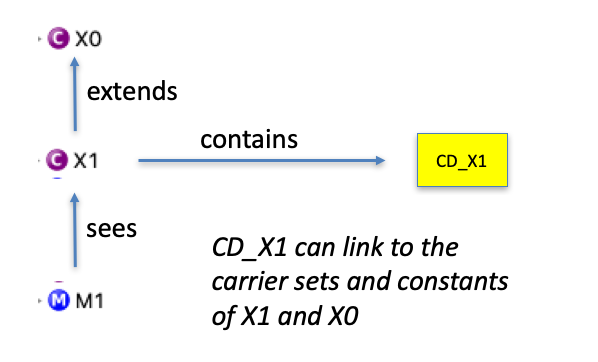
\includegraphics[width=.5\textwidth]{figures/containment_2.png}
		\fi
		\caption{Class Diagram contained in an extended Context}
		\label{fig:CDContainment2}
	\end{figure}
	
	
	\begin{figure}[!htbp]
		\centering
		\ifplastex
		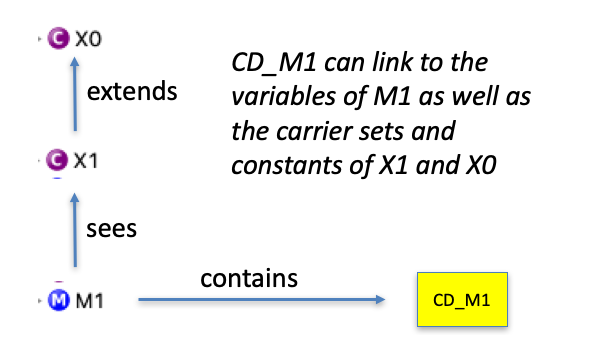
\includegraphics[width=500]{figures/containment_3.png}
		\else
		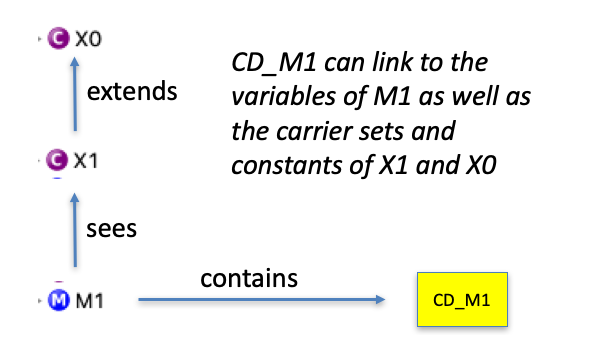
\includegraphics[width=.5\textwidth]{figures/containment_3.png}
		\fi
		\caption{Class Diagram contained in a Machine}
		\label{fig:CDContainment3}
	\end{figure}

%% subsections for each element type in a class diagram
	
	\section{Classes}
\label{sec:classdiagrams-classes}


	%
	\section{Class Attributes}
\label{sec:classdiagrams-attributes}



\paragraph{Initial Value } 
The initial value field is a Rodin Keyboard text field. 
The string in the text field is used as the intialisation value for the owning class attribute (or association) but can be interreted in several ways:
\begin{itemize}
	\item If the attribute is owned by a variable instance class, this field is currently ignored. (It should be used in a constructor).
	\item If the attribute elaborates a constant, this field is ignored. 
	\item If the attribute elaborates a variable, an action is added to the Initialisation event to intialise the attribute. as follows:
	\begin{itemize}
		\item if the text field begins with one of the Event-B assignment operators it is used to assign to the complete attribute relation (i.e. expression = attribute.name+initialValue.String)
		\item otherwise the text is assumed to contain the value to be assigned to each and every instance \\(i.e. expression = attribute.name+":="+class.name+"X"+initialValue.String)
	\end{itemize}	
\end{itemize}


%%% Local Variables:
%%% mode: latex
%%% TeX-master: "iuml-b-classdiagrams-user_manual"
%%% End:

	%
	\section{Associations}
\label{sec:classdiagrams-associations}


	%
	\section{Class Methods}
\label{sec:classdiagrams-methods}
	%
	\section{Class Constraints}
\label{sec:classdiagrams-constraints}

\begin{itemize}
	\item appropriate placement and deciding axiom or invariant

	\item quantification over instances

	\item considerations for ordering and how to fix it

\end{itemize}

	%
	\section{Class Statemachines}
\label{sec:classdiagrams-statemachines}
	
\end{document}

%%% Local Variables:
%%% mode: latex
%%% TeX-master: t
%%% End: